\section{Methods}
\subsection{Participants}
117 students were recruited between the 24.06.2024 and the 15.07.2024 from the university campus, with 83 (70.94\%) identifying as male, 34 (29.06\%) as female.
Participants were aged between 18 and 27, with a mean of 21.91 (\textit{SD} = 2.38) years, resulting in an interval of [19.53, 24.29].
Students of 32 study programs took part with the study programs most frequently represented being technical study programs, like Computer Science B.Sc. (n = 34), Software Engineering B.Sc. (n = 11), Aerospace Engineering B.Sc. (n = 8), Mechanical Engineering B.Sc. (n = 7) and Data Science B.Sc. (n = 5).
Participants gave informed consent, each received €15 as monetary compensation for their involvement in the study.

\subsection{Design}
This study employed a 2 $\times$ 8 factorial design, examining the impacts of gamified elements and gender on performance and anxiety \footnote{The study additionally incorporated concepts of motivation and self-efficacy, which, although not featured in my thesis, are included in the doctoral thesis of Nadine Koch} within a digital learning environment.
The independent variables were gamified elements and gender.
Gamified elements, included the following eight conditions: No Gamification (None), Points (P), Badges (B), Leaderboards (L), Avatars (A), Narrated Content (N), "Points, Badges, Leaderboards, Avatars" (PBLA) and "Points, Badges, Leaderboards, Avatars, Narrated Content" (PBLAN).
The gender variable was measured categorically with participants identifying as male or female.
Each participant experienced three blocks of a quiz with 20 items enhanced with  one different condition (gamified element), chosen randomly from a pre-generated set to ensure a balanced distribution across conditions and three questionnaires about it afterwards.
However, since each participant experienced only three out of the eight possible conditions, and different participants could experience different sets of conditions, this setup integrates elements of both within-subjects and between-subjects designs.
This allowed for the analysis of interaction effects between gamified elements and gender on the dependent variables, which were performance and anxiety.

\subsection{Materials}
\subsubsection{Physical Environment}
The study was conducted in two separate software laboratories in the cellar of a university building, one equipped with five and one with seven iMacs.
As \textcite{christyLeaderboardsVirtualClassroom2014} suggested that the environment can influence the results, both rooms were equipped with the same furniture and lighting and were furnished like a typical software laboratory.

\subsubsection{Virtual Environment}
The software used in this study was built by the author using SvelteKit in frontend and KTor in backend. Its UI was designed after the study by \textcite{albuquerqueDoesGenderStereotype2017}.
On the iMacs the study was displayed full-screen mode using the Safari web browser to ensure no further distractions. The study consisted of 7 pages.
A consent screen gave an overview and explained the data collection to the user. The consent screen had to be accepted in order to proceed.
The demographic data screen collected gender, age and study program. Participants also had to enter a deletion code in order to request their data's deletion after the collection.
%\begin{figure}[H]
%  \centering
%  \includegraphics[width=0.7\textwidth]{img/details.png}
%  \caption{The personal details collection form}
%  \label{fig:figureDetails}
%\end{figure}
A gamified learning environment, where the participants had to solve questions while being exposed to the gamified elements.
The matrices were taken from \textcite{albuquerqueDoesGenderStereotype2017}, for example \autoref{fig:figureMatrices} (left), to generate 60 questions out of the 20, the 40 questions for iteration two and three were slightly altered versions of the original 20 made by this author.
Those alterations included changing the position or rotation of the elements in the matrix and the five possible answers, for example \autoref{fig:figureMatrices} (right).
\begin{figure}[H]
  \centering
  \begin{subfigure}[t]{0.45\textwidth}
    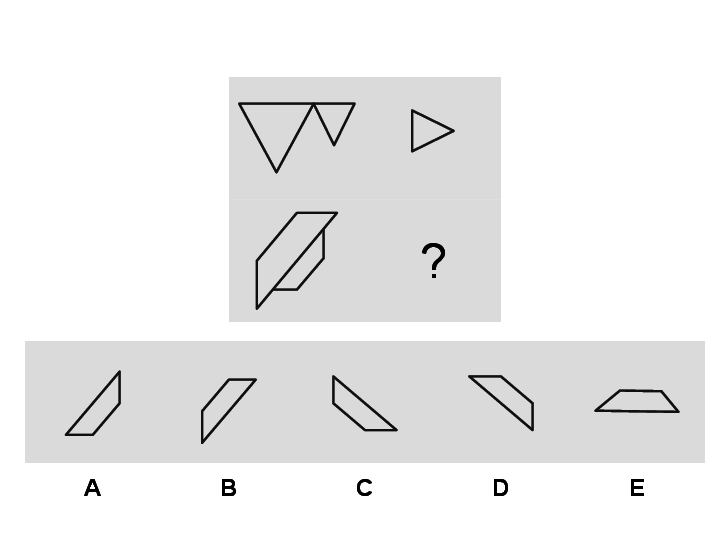
\includegraphics[width=\textwidth]{img/q-17.png}
  \end{subfigure}
  \hspace{5mm}
  \begin{subfigure}[t]{0.45\textwidth}
    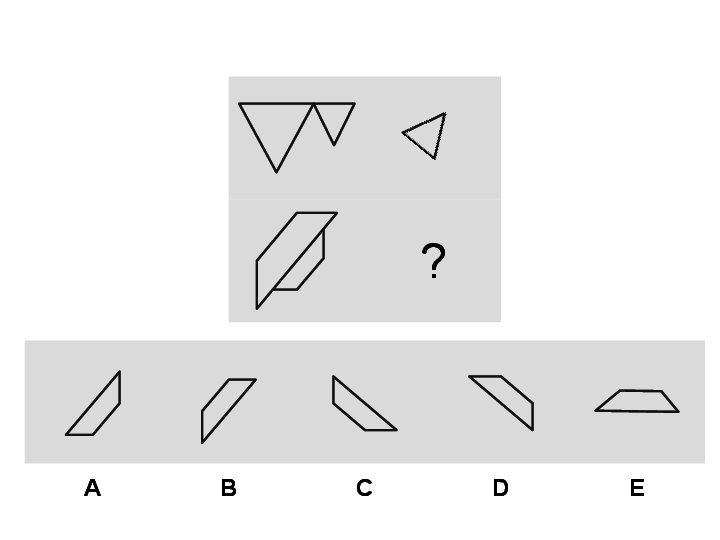
\includegraphics[width=\textwidth]{img/q-57.png}
  \end{subfigure}
  \caption{Left: A standard progressive matrix from \textcite{albuquerqueDoesGenderStereotype2017} shown in the quiz to the participants with D being the right answer. Right: A slightly altered version by rotating the top right triangle of the same matrix, changing the right answer to E.}
  \label{fig:figureMatrices}
\end{figure}
Tis gamified learning environment shown in \autoref{fig:figureScreen} consisted of different UI elements representing the gamified elements.
\begin{APAitemize}
  \item \textbf{Leaderboards}: A list of participants and scores, including the current participant. The list items consisted of rank, name in the format "Player " + random number and score, the players item was highlighted. The other players shown were not real, their scores were randomly generated so that the player started on the sixth place and the first place was always possible.
  \item \textbf{Badges}: An array of four badges that were awarded for 1, 5, 10 and 18 correctly answered questions.
  \item \textbf{Avatars}: A small avatar that was shown in the top right corner of the screen and on the leaderboard. To increase identification with the avatar further, the participants were asked to choose one of 15 different avatars before the iteration.
  \item \textbf{Narrated content}: Narrated content was shown in the bottom right corner of the screen. It was presented as a chat bubble with an avatar next to it, appearing like it spoke, in case avatars were enabled. It showed a random praise or encouragement sentence every three questions.
  \item \textbf{Points}: A counter next to the question frame showed the current points. One point was awarded for each correctly answered question.
\end{APAitemize}
\begin{figure}[H]
  \centering
  \begin{subfigure}[t]{\textwidth}
    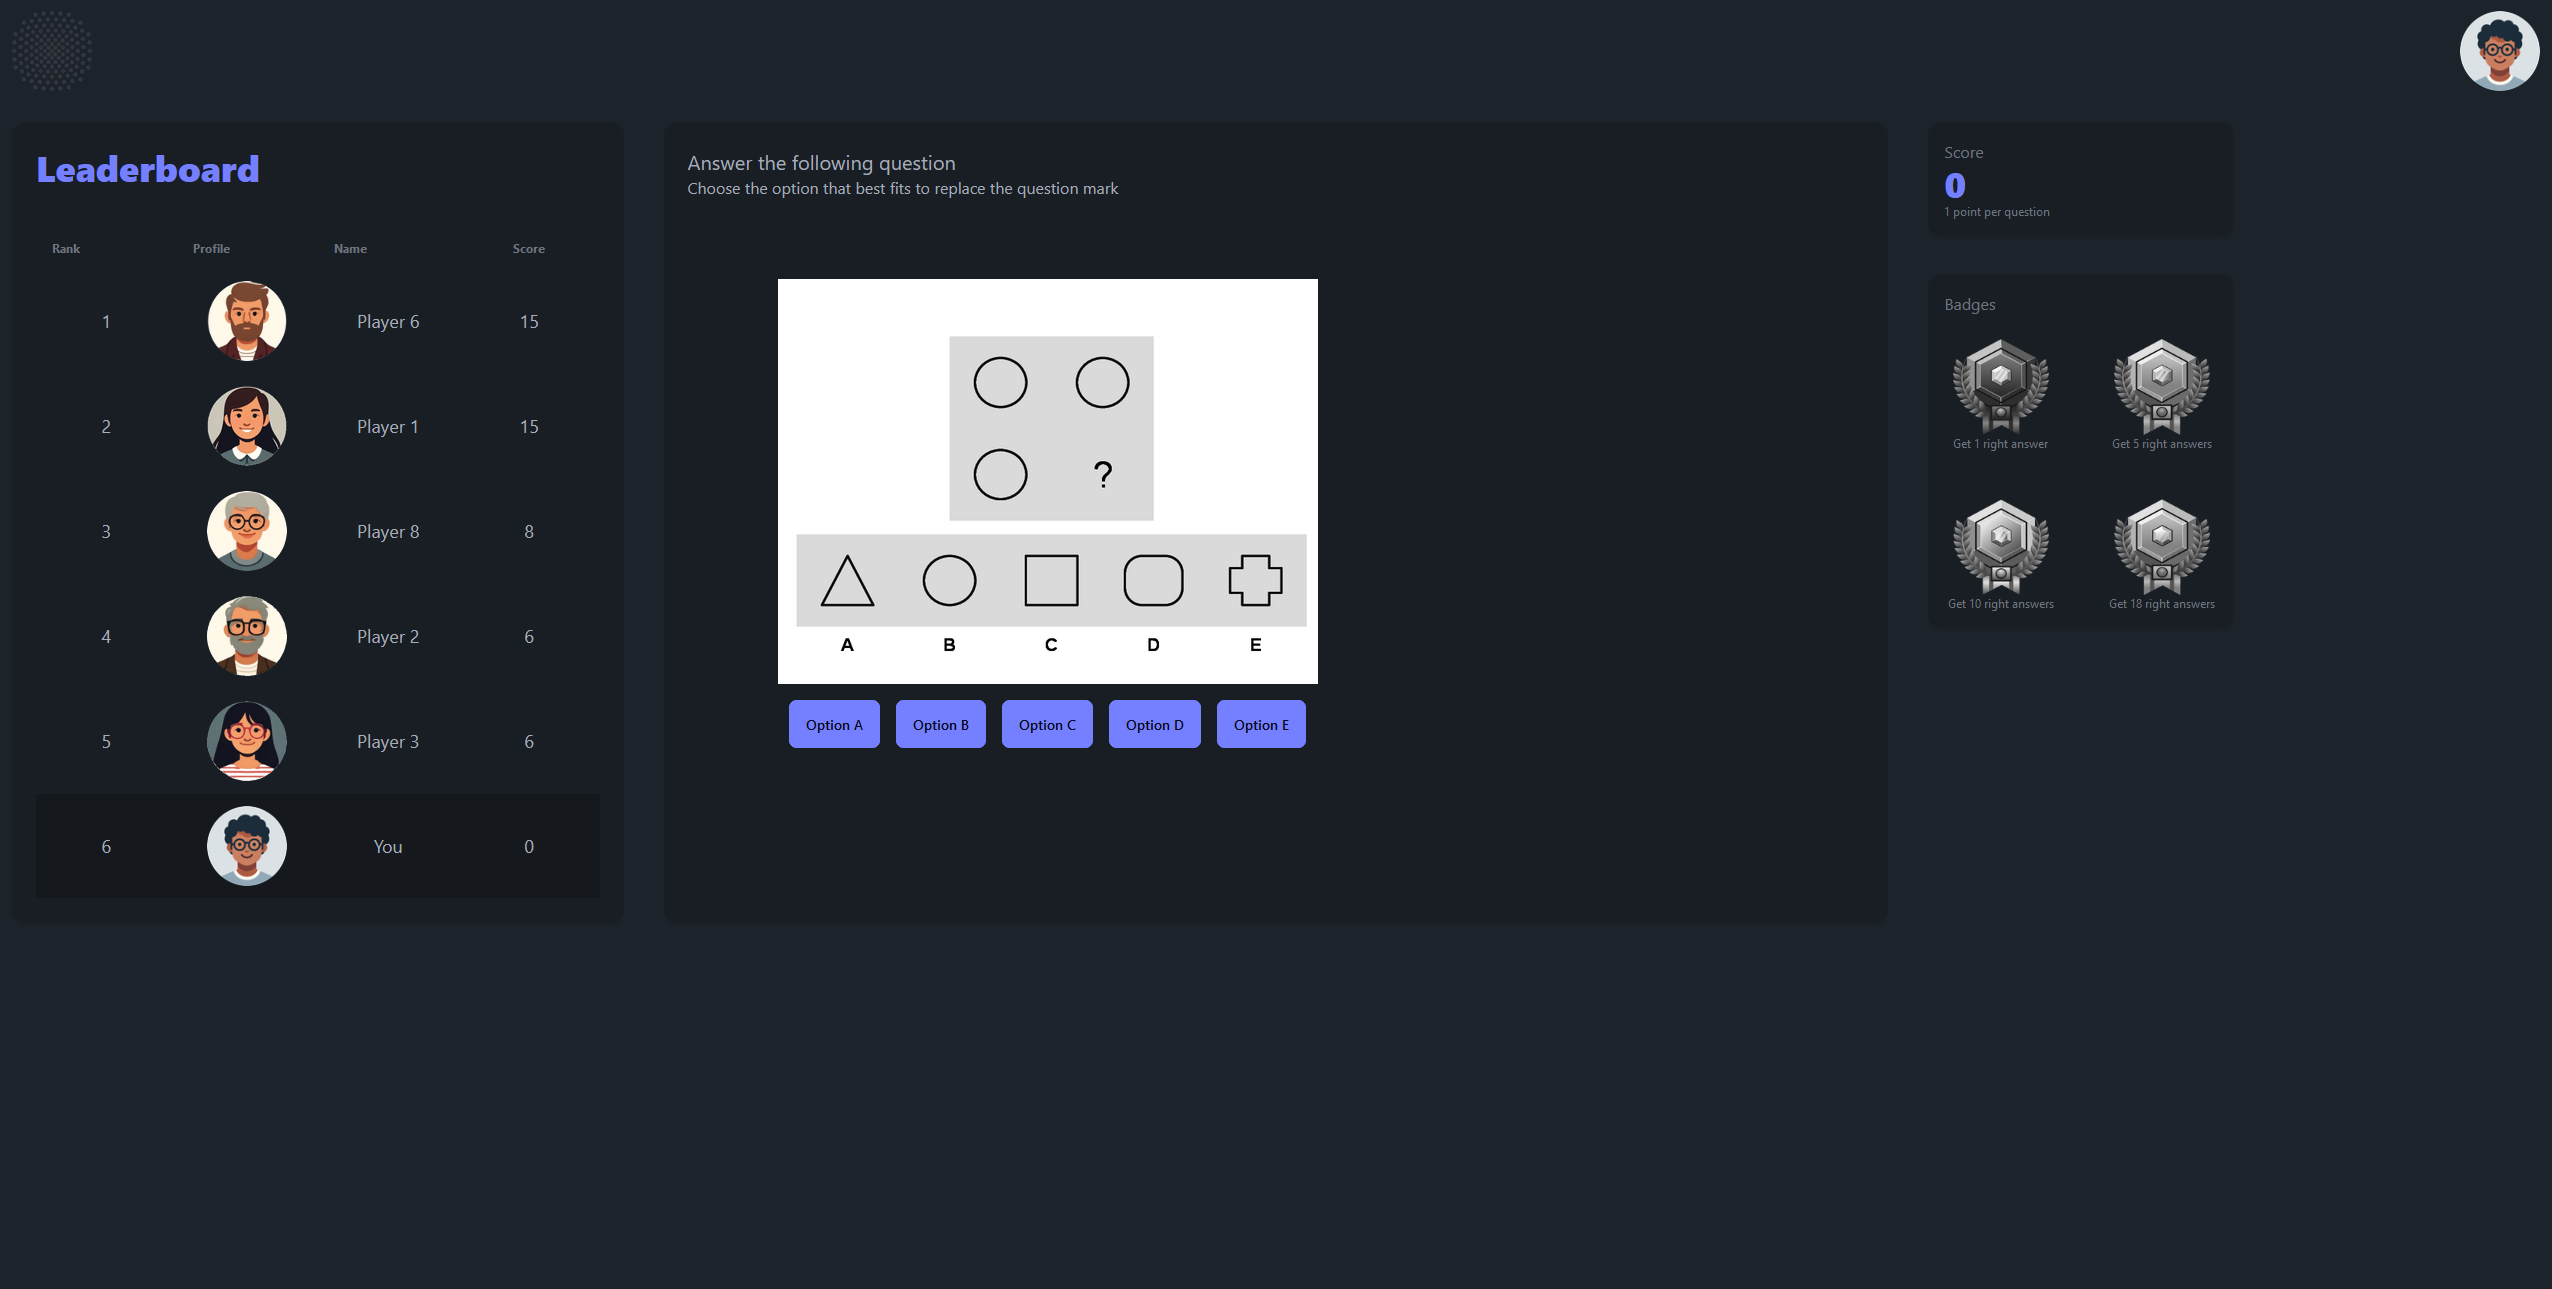
\includegraphics[width=\textwidth]{img/question_screen.png}
    \label{fig:figureScreenEnabled}
  \end{subfigure}
  \vspace{5mm}
  \begin{subfigure}[t]{\textwidth}
    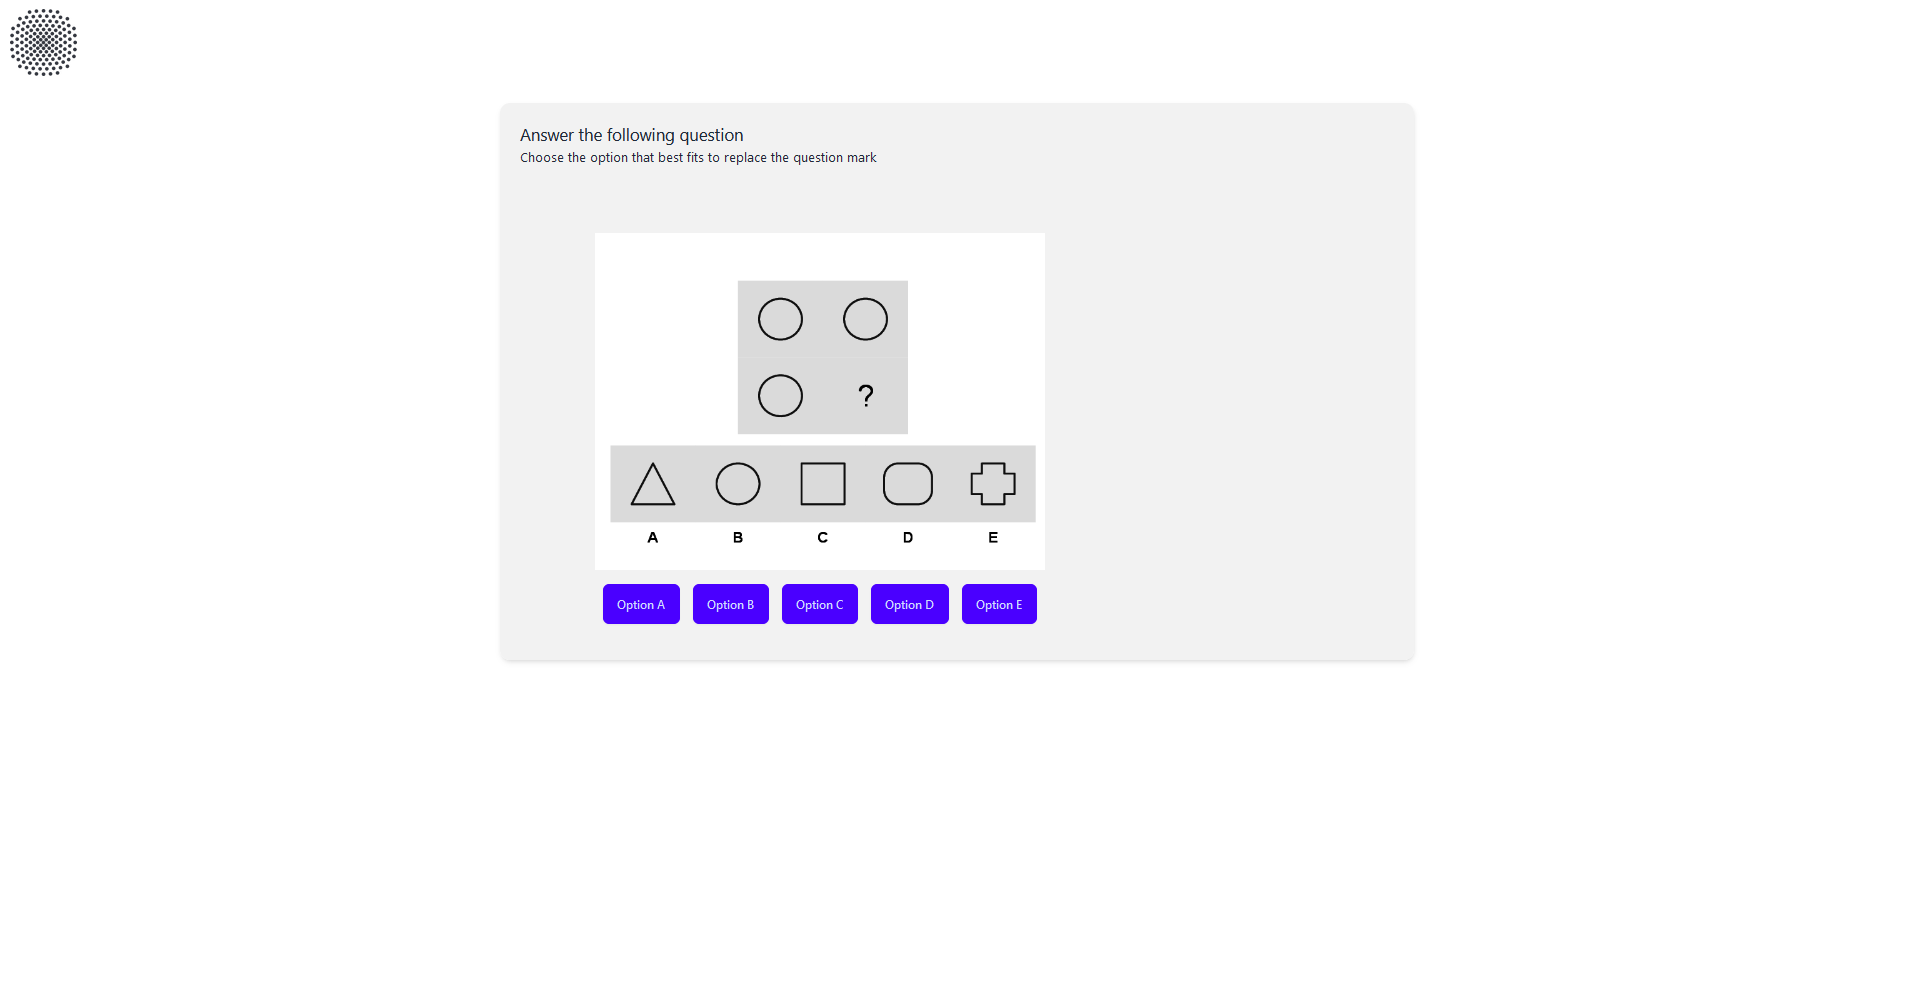
\includegraphics[width=\textwidth]{img/question_screen_no_elements.png}
    \label{fig:figureScreenDisabled}
  \end{subfigure}
  \caption{Comparison of the Digital Learning Environment with gamified elements enabled (left) and without gamified elements enabled (right). Narrated content in only shown between questions so it is not possible to show it in the same screenshot.}
  \label{fig:figureScreen}
\end{figure}

After the gamified learning environment, the participants were shown a questionnaire for anxiety, motivation and self-efficacy.
The three questionnaires were a six-question shortened form of the State-Trait Anxiety Inventory (STAI, \textcite{marteauDevelopmentSixitemShortform1992}), the eight-question General Self-Efficacy Scale (GSE \textcite{guayAssessmentSituationalIntrinsic2000}) and the 16-question Situational Intrinsic Motivation Scale (SIMS, \textcite{chenValidationNewGeneral2001}).
\begin{figure}[H]
  \centering
  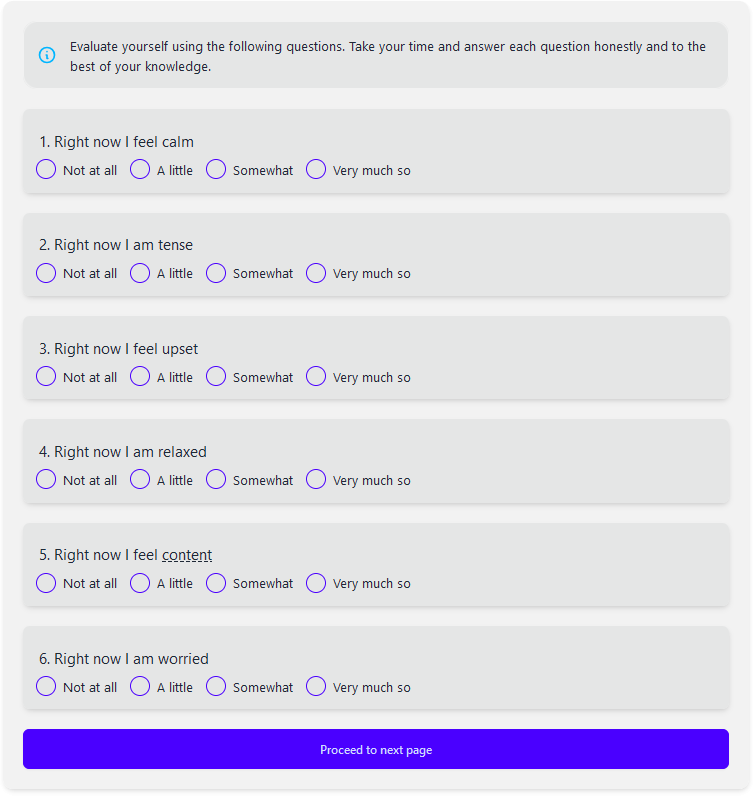
\includegraphics[width=0.7\textwidth]{img/Stai.png}
  \caption{The anxiety questionnaire with 6 items.}
  \label{fig:figureAnxiety}
\end{figure}
To submit data to the backend there was a data submission screen that guided the participants to the next iteration or in case of the third iteration to the end of the study.

\subsection{Procedure}
After a brief introduction to the study's framework, participants were instructed to to proceed at their own pace and were asked to avoid any communication with other participants throughout the study to prevent data contamination.
The initial interface they encountered obtained informed consent, followed by a screen to collect demographic information.
After entering their demographic data, participants progressed to the core of the study which consisted of three iterations of the gamified learning environment and the questionnaires afterward.
Each block began with a session in the gamified learning environment.
This was followed by the completion of the three questionnaires and each concluded with the data submission screen.
The transition between consecutive questions in the learning environment included a one-second delay, which extended to four seconds when narrated content was presented.
This standardized sequence ensured the reliability of the measurement process and comparability across different stages of the study.
After completing all three blocks, participants were thanked for their participation and compensated for their time.
\begin{figure}[H]
  \centering
  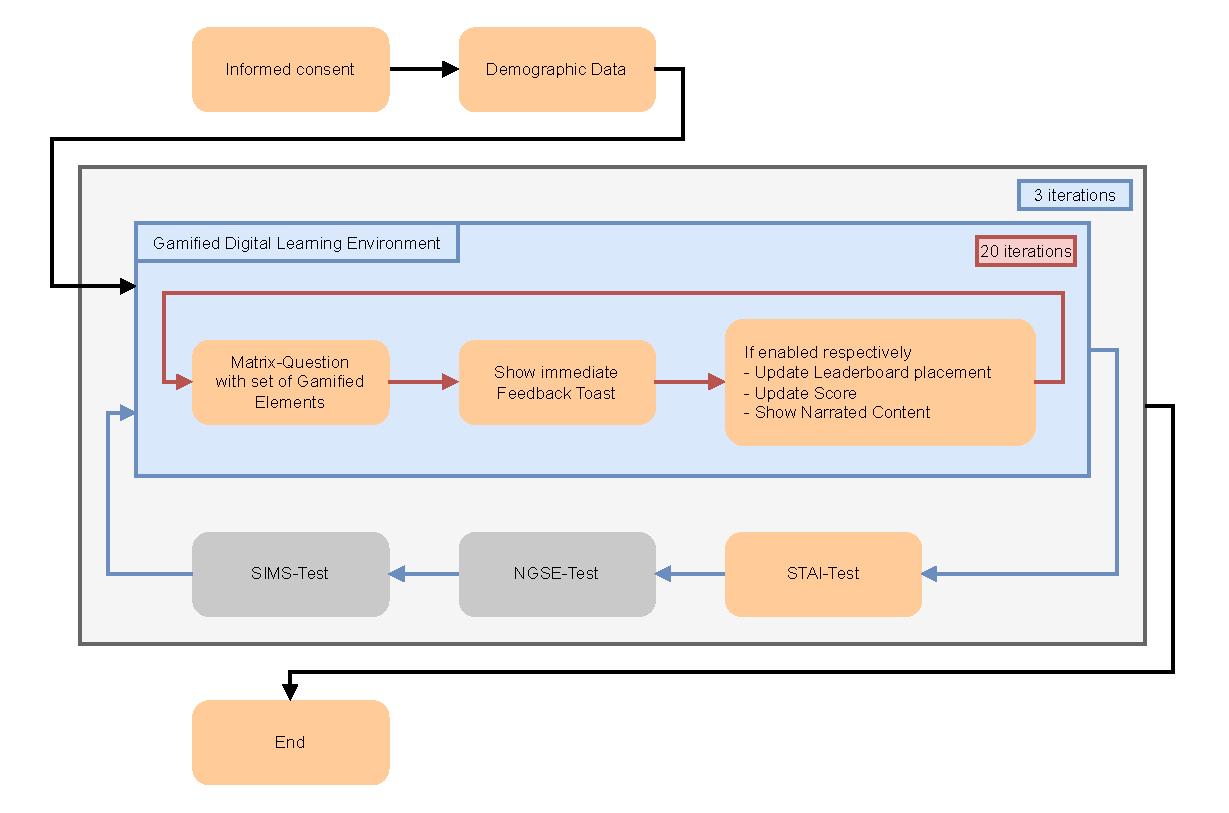
\includegraphics[width=\textwidth]{img/Procedure.pdf}
  \caption{Flowchart depicting the study procedure}
  \label{fig:procedureFlowchart}
\end{figure}


\subsection{Scoring}

The data was cleaned and processed before analysis to ensure accuracy and reliability. The scores for the different conditions were calculated as follows:

\begin{APAitemize}
\item \textbf{Performance:} The performance was calculated as the ratio of correctly answered questions to the total number of questions.
\item \textbf{State-Trait Anxiety Inventory (STAI):} The STAI scores were calculated using the six-item short-form version of the state scale, as developed by \textcite{marteauDevelopmentSixitemShortform1992}. Participants rated their responses on a scale from "Not at all" to "Very much so," corresponding to numerical values from one to four. The original test contains both anxiety-present and anxiety-absent items, with appropriate weights applied as per the guidelines by \textcite{courtMeasuringPatientAnxiety2010}. Negative weights were used for items indicating anxiety (e.g., "Right now I am worried"). The initial studies by \textcite{marteauDevelopmentSixitemShortform1992} reported a Cronbach's alpha of $0.82$ for the 6-item STAI, indicating good internal consistency. Subsequent Rasch analysis revealed an item separation reliability coefficient of $0.99$ and a person separation reliability coefficient of $0.78$, demonstrating the scale's refined measurement precision and ability to distinguish between varying anxiety levels \cite{courtMeasuringPatientAnxiety2010}.

\end{APAitemize}